\documentclass[11pt,a4paper]{report}
\usepackage[a4paper,margin=1in,headheight=15pt]{geometry}
\usepackage[T1]{fontenc}
\usepackage[utf8]{inputenc}
\usepackage{lmodern}
\usepackage{microtype}
\usepackage{xcolor}
\usepackage{booktabs}
\usepackage{tabularx}
\usepackage{longtable}
\usepackage{array}
\usepackage{enumitem}
\usepackage{amsmath,amssymb}
\usepackage{listings}
\usepackage{tikz}
\usetikzlibrary{arrows.meta,positioning,shapes.geometric}
\usepackage{fancyhdr}
\usepackage{lastpage}
\usepackage{titlesec}
\usepackage{hyperref}
\usepackage{bookmark}
\usepackage{parskip}
\usepackage{float}

\definecolor{navy}{HTML}{17365D}
\definecolor{blue}{HTML}{2563A6}
\definecolor{lightblue}{HTML}{EAF2F8}
\definecolor{lightgray}{HTML}{F3F5F7}
\definecolor{green}{HTML}{2E7D32}
\definecolor{orange}{HTML}{B85C00}
\hypersetup{colorlinks=true,linkcolor=navy,urlcolor=blue,pdftitle={DeepStoch Standard Operating Procedure},pdfauthor={DeepStoch Project Team}}
\pagestyle{fancy}
\fancyhf{}
\lhead{\textcolor{navy}{DeepStoch}}
\rhead{\textcolor{gray}{Standard Operating Procedure}}
\cfoot{\textcolor{gray}{Page \thepage\ of \pageref{LastPage}}}
\renewcommand{\headrulewidth}{0.4pt}
\renewcommand{\footrulewidth}{0.4pt}
\titleformat{\chapter}[display]{\normalfont\bfseries\color{navy}}{\chaptertitlename\ \thechapter}{8pt}{\Huge}
\titleformat{\section}{\normalfont\Large\bfseries\color{navy}}{\thesection}{0.75em}{}
\titleformat{\subsection}{\normalfont\large\bfseries\color{blue}}{\thesubsection}{0.75em}{}
\newcolumntype{Y}{>{\raggedright\arraybackslash}X}
\newcommand{\code}[1]{\texttt{\small #1}}
\lstset{basicstyle=\ttfamily\small,backgroundcolor=\color{lightgray},frame=single,breaklines=true,showstringspaces=false}

\begin{document}

\begin{titlepage}
\centering
\vspace*{1cm}
{\Large\textcolor{blue}{DISSERTATION SOFTWARE PROJECT}\par}
\vspace{1cm}
{\Huge\bfseries\textcolor{navy}{Standard Operating Procedure}\par}
\vspace{0.4cm}
{\LARGE\bfseries\textcolor{blue}{for DeepStoch}\par}
\vspace{0.8cm}
{\Large\itshape An Uncertainty-Aware Deep Learning and Stochastic Modelling Platform\par}
\vspace{1.2cm}
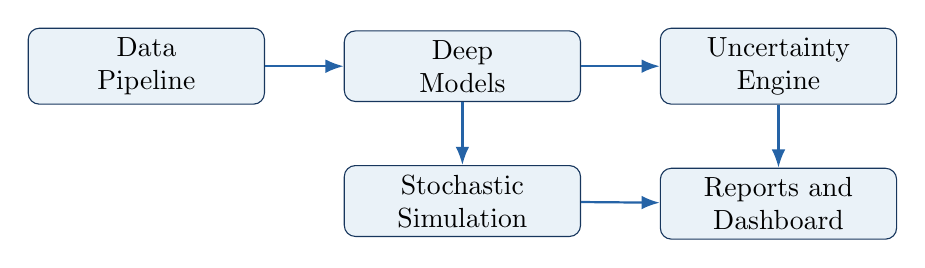
\begin{tikzpicture}[node distance=8mm and 10mm,>=Latex]
\node[draw=navy,fill=lightblue,rounded corners,minimum width=3cm,minimum height=0.8cm,align=center] (d) {Data\\Pipeline};
\node[draw=navy,fill=lightblue,rounded corners,minimum width=3cm,minimum height=0.8cm,align=center,right=of d] (m) {Deep\\Models};
\node[draw=navy,fill=lightblue,rounded corners,minimum width=3cm,minimum height=0.8cm,align=center,right=of m] (u) {Uncertainty\\Engine};
\node[draw=navy,fill=lightblue,rounded corners,minimum width=3cm,minimum height=0.8cm,align=center,below=of m] (s) {Stochastic\\Simulation};
\node[draw=navy,fill=lightblue,rounded corners,minimum width=3cm,minimum height=0.8cm,align=center,below=of u] (r) {Reports and\\Dashboard};
\draw[->,thick,blue] (d)--(m); \draw[->,thick,blue] (m)--(u); \draw[->,thick,blue] (m)--(s); \draw[->,thick,blue] (u)--(r); \draw[->,thick,blue] (s)--(r);
\end{tikzpicture}
\vfill
\begin{tabular}{>{\bfseries}p{4cm}p{7cm}}
Project & DeepStoch \\
Document & Standard Operating Procedure \\
Version & 1.0 - Dissertation Planning Release \\
Date & 23 October 2026 \\
Status & Controlled working document \\
\end{tabular}
\vfill
{\large Prepared for the DeepStoch long-term software project\par}
\end{titlepage}

\pagenumbering{roman}
\chapter*{Document Control}
\addcontentsline{toc}{chapter}{Document Control}
\begin{tabularx}{\textwidth}{>{\bfseries}p{3.5cm}Y}
Document identifier & DEEPSTOCH-SOP-001 \\
Owner & DeepStoch Project Team \\
Review cycle & Each major release and before dissertation submission \\
Primary use & Software construction, verification, and dissertation evidence \\
Repository & \code{D:\textbackslash Stochastic-Process-used-in-Software-reliability\textbackslash DeepStoch} \\
\end{tabularx}

\vspace{0.7cm}
\begin{tabularx}{\textwidth}{p{1.4cm}p{2.2cm}Y}
\toprule Version & Date & Change \\
\midrule 1.0 & 23 Oct 2026 & Initial DeepStoch SOP covering product definition, tools, models, methods, development, evaluation, and release control. \\
\bottomrule
\end{tabularx}

\tableofcontents
\clearpage
\pagenumbering{arabic}

\chapter{Purpose and Project Identity}

\section{Purpose}

This Standard Operating Procedure defines how DeepStoch will be designed, implemented, evaluated, documented, and released. It is a controlled working document for a long-term dissertation software project.

\section{Project definition}

DeepStoch is a modular platform combining deep neural networks, classical machine learning, stochastic processes, simulation, and uncertainty estimation. Its first application is probabilistic time-series forecasting. The long-term platform may support energy, traffic, cybersecurity, healthcare simulation, cloud workloads, and AI-agent monitoring.

\section{Dissertation objective}

\begin{quote}
To design and implement a modular software platform that combines neural forecasting with stochastic-process simulation and uncertainty estimation for data-driven decision support.
\end{quote}

The software must produce not only a prediction, but also an indication of uncertainty and, where appropriate, simulated future trajectories.

\section{Scope boundary}

The first dissertation release includes CSV time-series ingestion, data validation, chronological splitting, statistical and classical ML baselines, an LSTM or GRU model, probabilistic forecasts, Monte Carlo dropout or deep ensembles, stochastic simulation, anomaly scoring, experiment tracking, a dashboard, tests, and documentation.

The first release does not include training a foundation model, autonomous medical or financial decisions, unrestricted code execution, or production claims of guaranteed correctness.

\chapter{Objectives and Research Questions}

\section{Objectives}
\begin{enumerate}
\item Build an installable, modular, and reproducible software platform.
\item Compare simple, classical, neural, and probabilistic models.
\item Represent prediction uncertainty using transparent methods.
\item Implement reusable stochastic-process simulators.
\item Provide a dashboard for forecasts, uncertainty, simulation, and reports.
\item Preserve an evidence trail suitable for dissertation evaluation.
\end{enumerate}

\section{Research and engineering questions}
\begin{enumerate}
\item How can neural forecasting and stochastic simulation be exposed through one software architecture?
\item Which uncertainty methods produce useful and calibrated intervals?
\item How can the system detect when an input is unfamiliar or a prediction is unreliable?
\item How can advanced models be added without breaking reproducibility and evaluation contracts?
\item How can predictions be converted into scenario-based decision support?
\end{enumerate}

\chapter{System Architecture}

\section{Logical architecture}
\begin{figure}[H]
\centering
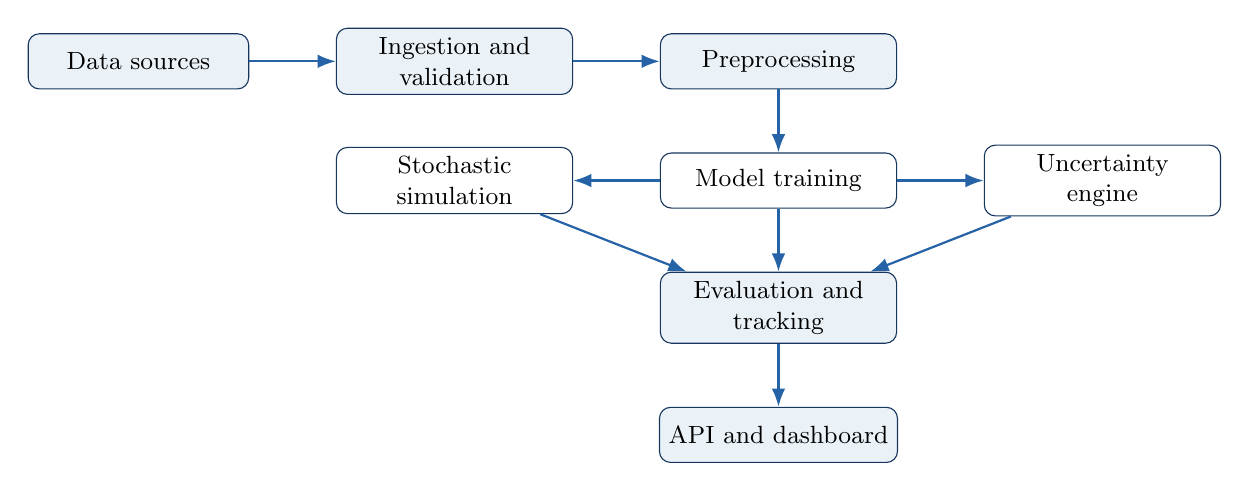
\begin{tikzpicture}[node distance=8mm and 11mm,>=Latex, every node/.style={font=\small}]
\node[draw=navy,fill=lightblue,rounded corners,minimum width=2.8cm,minimum height=0.7cm,align=center] (a) {Data sources};
\node[draw=navy,fill=lightblue,rounded corners,minimum width=3cm,minimum height=0.7cm,align=center,right=of a] (b) {Ingestion and\\validation};
\node[draw=navy,fill=lightblue,rounded corners,minimum width=3cm,minimum height=0.7cm,align=center,right=of b] (c) {Preprocessing};
\node[draw=navy,fill=white,rounded corners,minimum width=3cm,minimum height=0.7cm,align=center,below=of c] (d) {Model training};
\node[draw=navy,fill=white,rounded corners,minimum width=3cm,minimum height=0.7cm,align=center,left=of d] (e) {Stochastic\\simulation};
\node[draw=navy,fill=white,rounded corners,minimum width=3cm,minimum height=0.7cm,align=center,right=of d] (f) {Uncertainty\\engine};
\node[draw=navy,fill=lightblue,rounded corners,minimum width=3cm,minimum height=0.7cm,align=center,below=of d] (g) {Evaluation and\\tracking};
\node[draw=navy,fill=lightblue,rounded corners,minimum width=3cm,minimum height=0.7cm,align=center,below=of g] (h) {API and dashboard};
\draw[->,thick,blue] (a)--(b); \draw[->,thick,blue] (b)--(c); \draw[->,thick,blue] (c)--(d); \draw[->,thick,blue] (d)--(g); \draw[->,thick,blue] (e)--(g); \draw[->,thick,blue] (f)--(g); \draw[->,thick,blue] (d)--(f); \draw[->,thick,blue] (d)--(e); \draw[->,thick,blue] (g)--(h);
\end{tikzpicture}
\caption{Target architecture of DeepStoch.}
\end{figure}

\section{Software components}
\begin{longtable}{p{3.2cm}p{5cm}p{5.5cm}}
\toprule Component & Responsibility & Initial implementation \\
\midrule
Data layer & Load, validate, describe, and version data & pandas and custom validators \\
Feature pipeline & Scaling, imputation, windowing, and features & scikit-learn transformers \\
Model layer & Train and infer with multiple model families & scikit-learn and PyTorch adapters \\
Stochastic engine & Simulate Markov, Poisson, random-walk, and diffusion processes & NumPy, SciPy, and tested custom code \\
Uncertainty engine & Produce intervals, ensembles, and calibration & PyTorch and custom metrics \\
Evaluation engine & Compare models and report limitations & scikit-learn, SciPy, and custom metrics \\
Experiment service & Track configurations, metrics, and artifacts & MLflow \\
API and dashboard & User workflow and result visualization & FastAPI, React, TypeScript, Plotly \\
\bottomrule
\end{longtable}

\chapter{Tools and Development Environment}

\begin{tabularx}{\textwidth}{p{3cm}p{4cm}Y}
\toprule Tool & Role & DeepStoch use \\
\midrule
Python & Primary language & Data, models, simulations, APIs, and tests \\
NumPy and pandas & Numerical and tabular computing & Arrays, data cleaning, and time-series preparation \\
SciPy and statsmodels & Scientific and statistical computing & Distributions, optimization, diagnostics, and baselines \\
scikit-learn & Classical ML & Baselines, preprocessing, calibration, metrics, and anomaly detection \\
PyTorch & Deep learning & MLP, CNN, RNN, LSTM, GRU, ensembles, and future hybrid models \\
FastAPI and Pydantic & Backend and schemas & Dataset, training, inference, simulation, and reports \\
React and TypeScript & Frontend & Browser dashboard and user workflow \\
MLflow & MLOps & Run, metric, artifact, and model tracking \\
pytest, Ruff, mypy & Quality & Automated tests, linting, and type checks \\
Git and Docker & Reproducibility & Source history, packaging, and deployment environments \\
\bottomrule
\end{tabularx}

The initial environment shall be CPU-compatible. GPU acceleration may be introduced later for large ensembles, Transformer models, diffusion models, or neural stochastic differential equations.

\chapter{Mathematical and Model Methods}

\section{Stochastic processes}

The planned process library includes discrete and continuous-time Markov chains, Poisson and non-homogeneous Poisson processes, birth-death processes, random walks, Brownian motion, geometric Brownian motion, Ornstein-Uhlenbeck processes, hidden Markov models, state-space models, and stochastic differential equations.

For a finite-state Markov chain:
\[
P_{ij}=\Pr(X_{t+1}=j\mid X_t=i), \qquad \sum_jP_{ij}=1.
\]

For a Poisson process:
\[
\Pr\{N(t)=k\}=\frac{e^{-\lambda t}(\lambda t)^k}{k!}.
\]

For Brownian motion with drift:
\[
dX_t=\mu\,dt+\sigma\,dW_t.
\]

\section{Model progression}

The model ladder is:
\begin{enumerate}
\item mean, last-value, seasonal-naive, and moving-average baselines;
\item linear regression, exponential smoothing, ARIMA, random forest, and gradient boosting;
\item MLP, one-dimensional CNN, RNN, LSTM, and GRU;
\item quantile and distributional neural forecasting;
\item Monte Carlo dropout, deep ensembles, bootstrap, and conformal prediction;
\item temporal convolutional and Transformer models;
\item neural state-space models and neural SDEs.
\end{enumerate}

\section{Neural forecasting}

For a history window of length $L$ and horizon $H$, the first neural model will learn:
\[
\mathbf{x}_{t-L+1:t}\longmapsto \widehat{\mathbf{y}}_{t+1:t+H}.
\]

\section{Probabilistic forecasting}

For quantile level $\tau$, the pinball loss is:
\[
L_\tau(y,\widehat q_\tau)=
\begin{cases}
\tau(y-\widehat q_\tau), & y\geq\widehat q_\tau,\\
(1-\tau)(\widehat q_\tau-y), & y<\widehat q_\tau.
\end{cases}
\]

A distributional model may predict:
\[
Y_{t+h}\sim\mathcal{N}(\mu_{t+h},\sigma_{t+h}^2), \qquad \sigma_{t+h}>0.
\]

\section{Uncertainty estimation}

DeepStoch shall distinguish aleatoric uncertainty, epistemic uncertainty, and distribution-shift uncertainty. The practical implementation order is Monte Carlo dropout, deep ensembles, bootstrap, conformal prediction, calibration analysis, and out-of-distribution detection.

For repeated stochastic predictions $\widehat y^{(1)},\ldots,\widehat y^{(M)}$:
\[
\overline y=\frac{1}{M}\sum_{m=1}^M\widehat y^{(m)},
\qquad
s^2=\frac{1}{M-1}\sum_{m=1}^M(\widehat y^{(m)}-\overline y)^2.
\]

\chapter{Data and Experiment Procedure}

For every dataset record its source, access date, license, units, time field, target variable, missing-value meaning, and limitations. Validate format, schema, timestamps, duplicates, missing values, irregular intervals, target availability, and leakage.

Time-series data shall be split chronologically:
\[
\text{earlier period}\rightarrow\text{training},
\quad
\text{middle period}\rightarrow\text{validation},
\quad
\text{latest period}\rightarrow\text{test}.
\]

Every experiment shall record the dataset ID, preprocessing, model type, hyperparameters, random seed, code commit, hardware, training metrics, validation metrics, test metrics, plots, artifacts, and limitations. MLflow shall be used for run tracking.

\chapter{Evaluation and Quality Assurance}

Point forecasts shall use MAE, RMSE, mean error, residual analysis, and horizon-wise error. Probabilistic forecasts shall use negative log-likelihood, pinball loss, interval coverage, interval width, calibration error, and CRPS where implemented. Anomaly detection shall use precision, recall, F1, false-alarm rate, and detection delay.

Unit tests shall cover validators, preprocessing, windows, metrics, probability calculations, simulators, tensor shapes, and API schemas. Integration tests shall cover upload-to-validation, training-to-checkpoint, checkpoint-to-inference, forecast-to-uncertainty, simulation-to-results, and dashboard flows. A fixed demonstration dataset shall be used for regression tests.

Before release, the project shall verify file limits, path traversal protection, safe serialization, secret exclusion, input validation, and sandboxing for any future generated-code execution.

\chapter{Roadmap and Release Control}

\begin{longtable}{p{1cm}p{3.3cm}p{7.5cm}p{2.3cm}}
\toprule Phase & Name & Main deliverables & Gate \\
\midrule
0 & Foundation & Package, configuration, health check, tests, documentation & Installable \\
1 & Data foundation & CSV ingestion, validation, preprocessing, chronological split & Validated data \\
2 & Baselines & Statistical and classical ML models with metrics & Comparison \\
3 & Deep forecasting & LSTM or GRU, training, checkpoint, inference & Neural forecast \\
4 & Probabilistic output & Quantiles, intervals, coverage, calibration & Interval report \\
5 & Uncertainty & Dropout or ensembles, warnings, OOD analysis & Uncertainty report \\
6 & Simulation & Markov, Poisson, random-walk, Brownian, Monte Carlo & Scenario report \\
7 & Dashboard & Browser workflow and report export & Usable interface \\
8 & Hybrid research & Neural state-space or neural-SDE prototype & Advanced comparison \\
9 & Dissertation release & Freeze, verify, document, and archive evidence & Reproducible release \\
\bottomrule
\end{longtable}

The first 24 weeks are divided into setup, data foundation, baselines, neural forecasting, probabilistic output, uncertainty, stochastic simulation, and dashboard release. Advanced models are deferred until the first complete workflow is stable.

\chapter{Risks, Ethics, and Definition of Done}

\begin{tabularx}{\textwidth}{p{3.5cm}Y}
\toprule Risk & Control \\
\midrule
Scope expansion & Freeze v0.1 before adding advanced model families. \\
Data leakage & Chronological splits and explicit leakage checks. \\
Misleading uncertainty & Empirical coverage, interval width, and calibration reports. \\
Reproducibility failure & Track code, data, configuration, seed, and environment. \\
Limited computation & CPU-compatible first release and staged experiments. \\
Sensitive data & Use public or synthetic data unless governance approval exists. \\
Unsafe automation & Sandboxing, resource limits, and human review. \\
\bottomrule
\end{tabularx}

Predictions and simulations shall be labelled as estimates. DeepStoch shall not claim medical, financial, safety-critical, or guaranteed decision capability in the first release.

A feature is complete only when implementation, normal and invalid-input tests, manual verification, documentation, reproducible configuration, known limitations, and acceptance criteria are all recorded.

\chapter{Immediate Action Plan}

\begin{enumerate}
\item Create the repository structure.
\item Create the Python environment.
\item Install the editable package.
\item Run the health check and tests.
\item Select one public time-series dataset.
\item Implement CSV validation and metadata.
\item Implement a last-value baseline.
\item Add dataset and baseline tests.
\item Track the first experiment.
\item Archive the Phase 1 report.
\end{enumerate}

\appendix
\chapter{Initial Repository Layout}
\begin{lstlisting}
DeepStoch/
├── deepstoch/       Python package and CLI
├── models/          ML and deep-learning models
├── stochastic/      Stochastic-process implementations
├── uncertainty/     Uncertainty and calibration methods
├── evaluation/      Metrics and comparison
├── data/            Dataset metadata and local locations
├── experiments/     Configurations and run records
├── tests/            Automated tests
├── docs/             Technical documents
├── configs/          Versioned configuration
├── deepstoch_sop/   Editable LaTeX SOP
├── pyproject.toml
└── README.md
\end{lstlisting}

\end{document}

